%% LyX 2.0.8.1 created this file.  For more info, see http://www.lyx.org/.
%% Do not edit unless you really know what you are doing.
\documentclass[english]{article}
\usepackage[T1]{fontenc}
\usepackage[latin9]{inputenc}
\usepackage{graphicx}

\makeatletter

%%%%%%%%%%%%%%%%%%%%%%%%%%%%%% LyX specific LaTeX commands.
\providecommand{\LyX}{L\kern-.1667em\lower.25em\hbox{Y}\kern-.125emX\@}
%% Because html converters don't know tabularnewline
\providecommand{\tabularnewline}{\\}

%%%%%%%%%%%%%%%%%%%%%%%%%%%%%% Textclass specific LaTeX commands.
\newenvironment{lyxcode}
{\par\begin{list}{}{
\setlength{\rightmargin}{\leftmargin}
\setlength{\listparindent}{0pt}% needed for AMS classes
\raggedright
\setlength{\itemsep}{0pt}
\setlength{\parsep}{0pt}
\normalfont\ttfamily}%
 \item[]}
{\end{list}}

\makeatother

\usepackage{babel}
\begin{document}

\title{GenClass: A portable tool for data classification based on Grammatical
Evolution}


\author{Ioannis G. Tsoulos$^{(1)}$, Alexandros Tzallas$^{(1)}$, Dimitris
Tsalikakis$^{(2)}$}


\date{$^{(1)}$Department of Computer Engineering, School of Applied Technology,
Technological Educational Institute of Epirus, 47100 Arta, Greece
\\
$^{(2)}$University of Western Macedonia, Department of Engineering
Informatics and Telecommunications, Greece }
\maketitle
\begin{abstract}
A genetic programming based method is introduced for data classification.
The fundamental element of the method is the well - known technique
of Grammatical Evolution. The method constructs classification programs
in a C \textendash{} like programming language in order to classify
the input data, producing simple if \textendash{} else rules. The
paper introduces the method and the corresponding programming tool.
Also, the method is tested on a series of datasets against other well
known classification tools.
\end{abstract}
\textbf{Keywords}: Genetic algorithm; Data classification; Grammatical
evolution; Stochastic methods


\section{Introduction }

Data classification finds many applications on a series of practical
problems from areas such as chemistry \cite{key-1,key-2,key-7}, biology
\cite{key-3,key-8}, economics \cite{key-4,key-9}, physics \cite{key-5,key-6}
etc. During the past years many methods have been proposed to problems
of this category such as neural networks \cite{key-10}, radial basis
functions networks \cite{key-11}, support vector machines \cite{key-12},
etc. The proposed method constructs classification programs in a human
readable format using the technique of Grammatical Evolution \cite{key-13}.
Grammatical evolution is an evolutionary process that has been applied
with success in many areas such as music composition \cite{key-14},
economics \cite{key-15}, symbolic regression \cite{key-17}, robot
control \cite{key-18} and caching algorithms \cite{key-19}. The
proposed method does not require additional information from the objective
problem (such as derivatives) and it can be applied to any dataset
without restrictions to the dimensionality of the problem.

The rest of this article is organized as follows: in section \ref{sec:Method-description}
the basic steps of the method are outlined as well as the installation
steps for the relevant software. In section \ref{sec:Experimental-results}
a series of experiments on some well - known classification datasets
are demonstrated. In section \ref{sec:Conclusions} conclusions and
guidelines for further expansion of the software are presented. 


\section{Method description \label{sec:Method-description}}


\subsection{The proposed algorithm }

The procedure of Grammatical Evolution has two major requirements: 
\begin{itemize}
\item The context free grammar (CFG) of the target language as expressed
in Backus Naur Form (BNF ).
\item The associated fitness function. 
\end{itemize}
The CFG grammar $G$ is defined as $G=\left(N,T,S,P\right)$, where
$N$ is a set of non terminal symbols, $T$ is a finite set of terminal
symbols with the constraint $N\cap T=\emptyset$. The terminal symbol
$S$ is named start symbol of the grammar and $P$ is a finite set
of production rules in the form $A\rightarrow a$ or $A\rightarrow aB,\ A,B\in N,\ a\in T$.

Grammatical evolution is a genetic programming procedure, but the
chromosomes are not expressed in the usual for of parse trees but
as vectors of integers. Each element of the vector stands for a production
rule from the given BNF grammar. The procedure initiates from the
start symbol of the grammar and iteratively produces the program string,
by replacing non terminal symbols with the right hand of the selected
production rule. The selection is performed in two steps: 
\begin{itemize}
\item The next element from the vector is taken (denoted as V). 
\item The production rule is selected using the scheme Rule = V mod R, where
R is the number of production rules for the current non \textendash{}
terminal symbol. 
\end{itemize}
The selection is executed iteratively until either a valid expression
is produced or the end of chromosome is reached. For the second case
the chromosome is considered as invalid and we can start over (wrapping
event) from the beginning of the chromosome. If the maximum number
of wrapping events has been reached, then the chromosome is considered
as invalid. The BF grammar used in the software to create a classification
program for a problem with two classes (0 and 1) is shown in figure\textbf{
\ref{fig:The-grammar-used}}. The parameter D determines the dimensionality
of the objective problem. The numbers in parentheses denote the sequence
number of the corresponding production rule to be used in the chromosome
production procedure.\textbf{ }In the proposed technique the chromosomes
are represented as sets of integers rather than in binary form. This
representation was chosen to increase speed of the evolution. Each
gene $g_{i}$ is defined as: $g_{i}\in\left[0..255\right]$. The upper
limit 255 means that the maximum number of production rules in the
grammar is 255 but this limit can easily change. For better understanding
of the production procedure consider the chromosome $C=\left[10,65,12,31,28,9,8,6,10,6,2,0,1\right]$.
In table \ref{tab:Steps-of-producing} we list the steps of producing
a valid classification program using the grammar of two classes in
\ref{fig:The-grammar-used}. The dimensionality of the input problem
is considered as D=2 

The main steps of the algorithm are: 
\begin{enumerate}
\item \textbf{Initialization} step. 

\begin{enumerate}
\item Read the train data 
\item Set $N_{G}$ as the maximum number of generations
\item Set $N_{C}$ as the number of chromosomes in the population.
\item Set $P_{S}$ as the selection rate.
\item Set $P_{M}$ as the mutation rate.
\item Initialize the chromosomes of the population.\textbf{ }The chromosomes
are initialized randomly as vectors of integers. 
\end{enumerate}
\item \textbf{Genetic} step

\begin{enumerate}
\item \textbf{For} $i=1,\ldots,N_{g}$ \textbf{do}

\begin{enumerate}
\item \textbf{Create} for every chromosome in the population a classification
program using the previous procedure of grammatical evolution. Denote
this classification program as $C_{i}$
\item \textbf{Calculate} the fitness $f_{i}$ for every chromosome of the
population. The fitness is calculated according to the following equation
\begin{equation}
f_{i}=\sum_{i=1}^{M}\left(C_{i}\left(x_{i}\right)-t_{i}\right)^{2}
\end{equation}
where $M$ denotes the number of input patterns in train data, $x_{i}$
is the $i$ train pattern and $t_{i}$ is the desired output. 
\item \textbf{Apply} the selection procedure: The chromosomes are sorted
in descending order according to their fitness value. The first $\left(1-P_{s}\right)\times N_{c}$
chromosomes are copied intact to the next generations. The rest of
the chromosomes are produced using the crossover procedure. For every
new chromosome two chromosomes (parents) are selected from the old
population using tournament selection. The procedure of tournament
selection has as follows: A set of $N>1$ randomly selected chromosomes
is produced and the chromosome with the best fitness value in this
set is selected and the others are discarded. Each new individual
is produced from the two selected parent using the so - called one
point crossover. During one point crossover the parent chromosomes
are cut at a randomly selected point and their right-hand side subchromosomes
are exchanged as show in figure \ref{fig:onepointcrossover}. 
\item \textbf{Apply} the mutation procedure: For every element in each chromosome
a random number $r$ in range $\left[0,1\right]$ is produced. If
$r\le P_{M}$ then the corresponding element is randomly changed.
\end{enumerate}
\item \textbf{EndFor}
\end{enumerate}
\item \textbf{Evaluation} step

\begin{enumerate}
\item Create a classification program for the best chromosome in the population.
\item Apply the previous program to test set and report the induced error.
\end{enumerate}
\end{enumerate}

\subsection{Distribution }

The package is distributed in a tar.gz file named \texttt{GenClass.tar.gz}
and under UNIX systems the user must issue the following commands
to extract the associated files:
\begin{enumerate}
\item gunzip \texttt{GenClass.tar.gz}
\item tar xfv \texttt{GenClass.tar}
\end{enumerate}
These steps create a directory named \texttt{GenClass} with the following
contents:
\begin{enumerate}
\item \textbf{bin}: A directory which is initially empty. After compilation
of the package, it will contain the executable\textbf{ genclass }
\item \textbf{doc}: This directory contains the documentation of the package
(this file) in different formats: A \LyX{} file, A \LaTeX{} file and
a PostScript file.
\item \textbf{examples}: A directory that contains some test functions.
\item \textbf{include}: A directory which contains the header files for
all the classes of the package.
\item \textbf{src}: A directory containing the source files of the package.
\item \textbf{Makefile}: The input file to the \texttt{make} utility in
order to build the tool. Usually, the user does not need to change
this file.
\item \textbf{Makefile.inc}: The file that contains some configuration parameters,
such as the name of the C++ compiler etc. The user must edit and change
this file before installation.
\end{enumerate}

\subsection{Installation }

The following steps are required in order to build the tool:
\begin{enumerate}
\item Uncompress the tool as described in the previous section.
\item \texttt{cd GenClass }
\item Edit the file \texttt{Makefile.inc} and change (if needed) the configuration
parameters.
\item Type \texttt{make}.
\end{enumerate}
The parameters in \texttt{Makefile.inc} are the following:
\begin{enumerate}
\item \textbf{CXX}: It is the most important parameter. It specifies the
name of the C++ compiler. In most systems running the GNU C++ compiler
this parameter must be set to g++.
\item \textbf{ROOTDIR}: Is the location of the GenClass directory. 
\end{enumerate}

\subsection{The executable genclass}

The outcome of the compilation is the executable \texttt{genclass}
under the directory \texttt{bin}. The executable has the following
command line parameters:
\begin{enumerate}
\item \texttt{-h}:The program prints a help screen and afterwards the program
terminates.
\item \texttt{-c} \texttt{\textbf{count}}: The integer parameter \texttt{\textbf{count}}
determines the number of chromosomes for the genetic population. The
default value for this parameter is 500.
\item -g \textbf{gens}: The integer parameter \textbf{gens} determines the
maximum number of generations allowed for the genetic algorithm. The
default value is 200.
\item \texttt{-s} \texttt{\textbf{srate}}: The double parameter \texttt{\textbf{srate}}
specifies the selection rate used in the genetic algorithm. The default
value for this parameter is 0.10 (10\%).
\item \texttt{-m} \texttt{\textbf{mrate}}: The double parameter \texttt{\textbf{mrate}}
specifies the mutation rate used in the genetic algorithm. The default
value for this parameter is 0.05 (5\%).
\item -l \textbf{size}: The integer parameter \textbf{size} determines the
size of every chromosome in the genetic population. The default value
for this parameter is 100.
\item -p \textbf{train\_file}: The string parameter \textbf{train\_file
}specifies the file containing the points that will be used as train
data for the algorithm. The file should conform to the format outlined
in figure \ref{fig:Data-format.}. The integer value D determines
the dimensionality of the problem and the value M determines the number
of points in the file. Every subsequent line contains a pattern and
the final column is the real output (category) for this pattern. The
number of the classes is induced from the train file. The software
scans the file and identifies the number of problem\textquoteright{}s
classes. The classes should be integer numbers with number 0 assigned
to the first class.
\item -t \textbf{test\_file}: The string parameter \textbf{test\_file }specifies
the file containing the test data for the particular problem. The
file should be in the same format as the \textbf{train\_file}.
\item -w \textbf{wrapping}. The integer parameter \textbf{wrapping} determines
the maximum number of wrapping events allowed. The default value for
this parameter is 1.
\item -f \textbf{foldcount}. The integer parameter \textbf{foldcount} specifies
the number of fold to be used for cross validation. The default value
for this parameter is 0 (no cross validation).
\item -o \textbf{method}: The string parameter method specifies the output
method for the executable. The available options are

\begin{enumerate}
\item simple. The program prints output only on termination. 
\item csv. The program prints in csv (comma separated value) format information
in every generation. In every generation the program prints: number
of generations, train error and test error. This is the default value
for the string parameter \textbf{method}.
\item full. The program prints in every generation detailed information
about the optimization procedure as well as classification error for
every distinct class of the problem.
\end{enumerate}
\item \texttt{-r} \texttt{\textbf{seed}}: The integer parameter \texttt{\textbf{seed}}
specifies the seed for the random number generator. It can assume
any integer value.
\end{enumerate}

\section{Experimental results \label{sec:Experimental-results}}


\subsection{A typical example }

Consider the Ionosphere dataset available from the Machine Learning
Repository in the following URL: http://www.ics.uci.edu/\textasciitilde{}mlearn/MLRepository.html.
The ionosphere dataset contains data from the Johns Hopkins Ionosphere
database. The two-class dataset contains 351 examples of 34 features
each. The datasets has been divided into two files, \texttt{ionosphere.train}
and \texttt{ionosphere.test} under directory \texttt{examples}. A
typical run for the \texttt{GenClass} will be
\begin{lyxcode}
../bin/genclass~-p~ionosphere.train~-t~ionosphere.test~-g~10~-o~csv
\end{lyxcode}
The output of this command is shown in figure \ref{alg:Typical-output-of}.


\subsection{Experiments}

In order to measure the efficiency of the proposed method a series
of experiments were conducted on some common classification problems
as well as two real world problems (EEG and Regions). For all the
experiments we have used 10-fold and they were conducted 30 times
using different seed for the random generator each time and averages
were taken. In all experiments we have used the parameters shown in
table \ref{tab:Parameters-for-the}. The following datasets were used 
\begin{enumerate}
\item Wine dataset. The wine recognition dataset contains data from wine
chemical analysis. It contains 178 examples of 13 features each that
are classified into three classes. 
\item Glass dataset. The dataset contains glass component analysis for glass
pieces that belong to 6 classes. The dataset contains 214 examples
with 10 attributes each.
\item Pima dataset. The Pima Indians Diabetes dataset contains 768 examples
of 8 attributes each that are classified into two categories: healthy
and diabetic.
\item Ionosphere dataset. The ionosphere dataset (ION in the following tables)
contains data from the Johns Hopkins Ionosphere database. The two-class
dataset contains 351 examples of 34 features each. 
\item Eeg dataset. As an real word example, consider an EEG dataset described
in \cite{key-20} is used here. The dataset consists of five sets
(denoted as Z, O, N, F and S) each containing 100 single-channel EEG
segments each having 23.6 sec duration. Sets Z and O have been taken
from surface EEG recordings of five healthy volunteers with eye open
and closed, respectively. Signals in two sets have been measured in
seizure-free intervals from five patients in the epileptogenic zone
(F) and from the hippocampal formation of the opposite hemisphere
of the brain (N). Set S contains seizure activity, selected from all
recording sites exhibiting ictal activity. Sets Z and O have been
recorded extracranially, whereas sets N, F and S have been recorded
intracranially.
\item Spiral artificial data: The spiral artificial dataset (SPIRAL) contains
1000 two-dimensional examples that belong to two classes (500 examples
each). The number of the features is 2. The data in the first class
are created using the following formula: $x_{1}=0.5t\cos\left(0.08t\right),\ x_{2}=0.5t\cos\left(0.08t+\frac{\pi}{2}\right)$
and the second class data using\textbf{: $x_{1}=0.5t\cos\left(0.08t+\pi\right),\ x_{2}=0.5t\cos\left(0.08t+\frac{3\pi}{2}\right)$}
\item Wisconsin diagnostic breast cancer: The Wisconsin diagnostic breast
cancer dataset (WDBC) contains data for breast tumors. It contains
569 training examples of 30 features each that are classified into
two categories.
\item Fertility Data Set (FERT): 100 volunteers provide a semen sample analyzed
according to the WHO 2010 criteria. Sperm concentration are related
to socio-demographic data, environmental factors, health status, and
life habits. It contains 100 examples of 10 features each.
\item Regions Data Set:Regions Dataset is created from liver biopsy images
of patients with hepatitis C \cite{Regions}. From each region in
the acquired images 18 shape-based and color-based features were extracted,
while it was also annotated form medical experts. The resulting dataset
includes 600 samples belonging into 6 classes.
\end{enumerate}
The results from the experiments are displayed in table \ref{tab:Experimental-results}.
The column DATASET denotes the name of the dataset. The column NEURAL
stands for the average test error from the application of neural network
to the corresponding dataset. The number of weights (hidden nodes)
for the neural network was set to 10 and a BFGS variant due to Powell
\cite{Powell} was used to train the network. The column RBF denotes
the average test error from the application of a Radial Basis Function
network to the dataset. In RBF network the hidden-layer weights are
estimated using the K-means algorithm and the pseudo-inverse method
is used to derive the output-layer weights The number of hidden nodes
for this network was also set to 10. Finally, the column GENCLASS
denotes the average test error from the application of the proposed
method to the dataset. As it can be deduced from the results, the
proposed can improve classification accuracy in the majority of the
used datasets. 


\section{Conclusions \label{sec:Conclusions}}

A software which implements a method for data classifications was
introduced. The method is based on grammatical evolution and the software
is designed to be portable. The software is entirely written in ANSI
C++ and there is not any specific software requirement. Future versions
of the software will include 
\begin{itemize}
\item Input from various formats.
\item Usage of improvement stopping rules for the genetic algorithm.
\item Additional output formats. \end{itemize}
\begin{thebibliography}{10}
\bibitem{key-1}C. G�ler, G. D. Thyne, J. E. McCray, K.A. Turner,
Evaluation of graphical and multivariate statistical methods for classification
of water chemistry data, Hydrogeology Journal \textbf{10}, pp. 455-474,
2002

\bibitem{key-2}E. Byvatov ,U. Fechner ,J. Sadowski , G. Schneider,
Comparison of Support Vector Machine and Artificial Neural Network
Systems for Drug/Nondrug Classification, J. Chem. Inf. Comput. Sci.
\textbf{43}, pp 1882\textendash{}1889, 2003.

\bibitem{key-7}Kunwar P. Singh, Ankita Basant, Amrita Malik, Gunja
Jain, Artificial neural network modeling of the river water quality\textemdash{}A
case study, Ecological Modelling \textbf{220}, pp. 888-895, 2009.

\bibitem{key-3}I. Guyon, J. Weston, S. Barnhill, V. Vapnik, Gene
Selection for Cancer Classification using Support Vector Machines,
Machine Learning \textbf{46}, pp. 389-422, 2002.

\bibitem{key-8}R. Marabini, J.M. Carazo, Pattern recognition and
classification of images of biological macromolecules using artificial
neural networks, Biophysical Journal \textbf{66}, pp. 1804-1814, 1994.

\bibitem{key-4}I. Kaastra, M. Boyd, Designing a neural network for
forecasting financial and economic time series, Neurocomputing \textbf{10},
pp. 215-236, 1996. 

\bibitem{key-9}Moshe Leshno, Yishay Spector, Neural network prediction
analysis: The bankruptcy case, Neurocomputing \textbf{10}, pp. 125-147,
1996.

\bibitem{key-5}S. R. Folkes,O. Lahav, S. J. Maddox, An artificial
neural network approach to the classification of galaxy spectra, Montly
Notices of the Royal Astronomical Society 283, pp 651-665, 1996. 

\bibitem{key-6}C.Z. Cai, W.L. Wang, Y.Z. Chen, Support vector machine
classification of physical and biological datasets, Int. J. Mod. Phys.
C 14, pp. 575, 2003

\bibitem{key-10}K. Hornik, Multilayer feedforward networks are universal
approximators, Neural Networks 2, pp. 359-366, 1989

\bibitem{key-11}M.D. Buhmann, Radial basis functions, Cambridge monographs
on Applied and Computational Mathemetics, 2003.

\bibitem{key-12}I. Steinwart, A. Christmann, Support Vector Machines,
Information Science and Statistics, Springer, 2008.

\bibitem{key-13}M. O\textquoteright{}Neill, C. Ryan, Grammatical
evolution, IEEE Trans. Evol. Comput. 5 (2001) 349\textendash{}358.

\bibitem{key-14}Alfonso Ortega, Rafael S�nchez, Manuel Alfonseca
Moreno, Automatic composition of music by means of grammatical evolution,
APL '02 Proceedings of the 2002 conference on APL: array processing
languages: lore, problems, and applications Pages 148 - 155.

\bibitem{key-15}Michael O\textquoteright{}Neill, Anthony Brabazon,
Conor Ryan, J. J. Collins, Evolving Market Index Trading Rules Using
Grammatical Evolution, Applications of Evolutionary Computing Volume
2037 of the series Lecture Notes in Computer Science pp 343-352. 

\bibitem{key-17}M. O\textquoteright{}Neill, C. Ryan, Grammatical
Evolution: Evolutionary Automatic Programming in a Arbitary Language,
Genetic Programming, vol. 4, Kluwer Academic Publishers, Dordrecht,
2003

\bibitem{key-18}J.J. Collins, C. Ryan, in: Proceedings of AROB 2000,
Fifth International Symposium on Artificial Life and Robotics, 2000.

\bibitem{key-19}M. O\textquoteright{}Neill, C. Ryan, in: K. Miettinen,
M.M. Mkel, P. Neittaanmki, J. Periaux (Eds.), Evolutionary Algorithms
in Engineering and Computer Science, Jyvskyl, Finland, 1999, pp. 127\textendash{}134.

\bibitem{key-20}R.G. Andrzejak, K. Lehnertz, F. Mormann, C. Rieke,
P. David, and C. E. Elger, Indications of nonlinear deterministic
and finite-dimensional structures in time series of brain electrical
activity: Dependence on recording region and brain state, Phys. Rev.
E \textbf{64}, pp. 1-8, 2001.

\bibitem{Powell}M.J.D. Powell, A Tolerant Algorithm for Linearly
Constrained Optimization Calculations, Mathematical Programming 45,
pp 547, 1989.

\bibitem{Regions}Giannakeas, N., Tsipouras, M.G., Tzallas, A.T.,
Kyriakidi, K., Tsianou, Z.E., Manousou, P., Hall, A., Karvounis, E.C.,
Tsianos, V., Tsianos, E. A clustering based method for collagen proportional
area extraction in liver biopsy images (2015) Proceedings of the Annual
International Conference of the IEEE Engineering in Medicine and Biology
Society, EMBS, 2015-November, art. no. 7319047, pp. 3097-3100. 

\end{thebibliography}
\begin{figure}
\caption{The grammar used by GenClass for a problem with two classes (0 and
1). The parameter D in the determination of non -terminal symbol XLIST
specifies the dimensionality of the objective problem. The numbers
in parentheses denote the sequence number of the corresponding production
rule to be used in the chromosome production procedure.\label{fig:The-grammar-used}}

\begin{lyxcode}
<S>::=if(<BEXPR>)~CLASS=0~else~CLASS=1~(0)



<BEXPR>::=<XLIST><BOOLOP><EXPR>~~~~~~~~~~~~(0)

~~~~~~~~~|!(<BEXPR>)~~~~~~~~~~~~~~~~~~~~~~~(1)

~~~~~~~~~|<XLIST><BOOLOP><EXPR>\&<BEXPR>~~~~(2)

~~~~~~~~~|<XLIST><BOOLOP><EXPR>|<BEXPR>~~~~(3)



<BOOLOP>::=~>~~~~~~~~~~~~~~~~~~~~~~~~~~~~~~(0)

~~~~~~~~~~|~>=~~~~~~~~~~~~~~~~~~~~~~~~~~~~~(1)

~~~~~~~~~~|~<~~~~~~~~~~~~~~~~~~~~~~~~~~~~~~(2)

~~~~~~~~~~|~<=~~~~~~~~~~~~~~~~~~~~~~~~~~~~~(3)

~

<EXPR>::=~(<EXPR><BINARYOP><EXPR>)~~~~~~~~~(0)

~~~~~~~~|~<FUNCTION>(<EXPR>)~~~~~~~~~~~~~~~(1)

~~~~~~~~|~<TERMINAL>~~~~~~~~~~~~~~~~~~~~~~~(2)



<BINARYOP>::=~+~~~~~~~~~~~~~~~~~~~~~~~~~~~~(0)

~~~~~~~~~~~~|~-~~~~~~~~~~~~~~~~~~~~~~~~~~~~(1)

~~~~~~~~~~~~|~{*}~~~~~~~~~~~~~~~~~~~~~~~~~~~~(2)

~~~~~~~~~~~~|~/~~~~~~~~~~~~~~~~~~~~~~~~~~~~(3)



<FUNCTION>::=~sin~|~cos~|~exp~|~log~~~~~~~~(0-3)



<TERMINAL>::=~<XLIST>~~~~~~~~~~~~~~~~~~~~~~(0)

~~~~~~~~~~~~|~<DIGITLIST>.<DIGITLIST>~~~~~~(1)

~~~~~~~~~~~~|~(-<DIGITLIST>.<DIGITLIST>)~~~(2)



~<XLIST>::=~x1~|~x2~|~...|xD~~~~~~~~~~~~~~~(0-D-1)



<DIGITLIST>::=<DIGIT>~~~~~~~~~~~~~~~~~~~~~~(0)

~~~~~~~~~~~~~|~<DIGIT><DIGIT>~~~~~~~~~~~~~~(1)

~~~~~~~~~~~~~|~<DIGIT><DIGIT><DIGIT>~~~~~~~(2)



<DIGIT>::=~0~|~1~|~2~|~3~|~4~|5~|6~|7~|8~|9~~~~(0-9)

\end{lyxcode}
\end{figure}
\begin{table}


\caption{Steps of producing an example valid classification program.\label{tab:Steps-of-producing} }


\raggedright{}%
\begin{tabular}{|c|c|c|}
\hline 
{\tiny{}String} & {\tiny{}Chromosome} & {\tiny{}Operation}\tabularnewline
\hline 
\hline 
{\tiny{}if(<BEXPR>) CLASS=0 else CLASS=1} & {\tiny{}10,65,12,31,28,9,8,6,10,6,2,0,1} & \tabularnewline
\hline 
{\tiny{}if(<XLIST><BOOLOP><EXPR>) CLASS=0 else CLASS=1} & {\tiny{}65,12,31,28,9,8,6,10,6,2,0,1} & {\tiny{}10\%4=0}\tabularnewline
\hline 
{\tiny{}if(x1<BOOLOP><EXPR>) CLASS=0 else CLASS=1} & {\tiny{}12,31,28,9,8,6,10,6,2,0,1} & {\tiny{}65\%2=1}\tabularnewline
\hline 
{\tiny{}if(x1><EXPR>) CLASS=0 else CLASS=1} & {\tiny{}31,28,9,8,6,10,6,2,0,1} & {\tiny{}12\%4=0}\tabularnewline
\hline 
{\tiny{}if(x1><EXPR><BINARYOP><EXPR>) CLASS=0 else CLASS=1} & {\tiny{}28,9,8,6,10,6,2,0,1} & {\tiny{}31\%3=1}\tabularnewline
\hline 
{\tiny{}if(x1><FUNCTION>(<EXPR)<BINARYOP><EXPR>) CLASS=0 else CLASS=1} & {\tiny{}9,8,6,10,6,2,0,1} & {\tiny{}28\%3=1}\tabularnewline
\hline 
{\tiny{}if(x1>cos(<EXPR>)<BINARYOP><EXPR>) CLASS=0 else CLASS=1} & {\tiny{}8,6,10,6,2,0,1} & {\tiny{}9\%4=1}\tabularnewline
\hline 
{\tiny{}if(x1>cos(<TERMINAL><BINARYOP><EXPR) CLASS=0 else CLASS=1} & {\tiny{}6,10,6,2,0,1} & {\tiny{}8\%3=2}\tabularnewline
\hline 
{\tiny{}if(x1>cos(<XLIST>)<BINARYOP><EXPR) CLASS=0 else CLASS=1} & {\tiny{}10,6,2,0,1} & {\tiny{}6\%3=0}\tabularnewline
\hline 
{\tiny{}if(x1>cos(x0)<BINARYOP><EXPR>) CLASS=0 else CLASS=1} & {\tiny{}6,2,0,1} & {\tiny{}10\%2=0}\tabularnewline
\hline 
{\tiny{}if(x1>cos(x0){*}<EXPR>) CLASS=0 else CLASS=1} & {\tiny{}2,0,1} & {\tiny{}6\%4=2}\tabularnewline
\hline 
{\tiny{}if(x1>cos(x0){*}<TERMINAL>) CLASS=0 else CLASS=1} & {\tiny{}0,1} & {\tiny{}2\%3=2}\tabularnewline
\hline 
{\tiny{}if(x1>cos(x0){*}<XLIST>) CLASS=0 else CLASS=1} & {\tiny{}1} & {\tiny{}0\%3=0}\tabularnewline
\hline 
{\tiny{}if(x1>cos(x0){*}x1) CLASS=0 else CLASS=1} &  & {\tiny{}1\%2=1}\tabularnewline
\hline 
\end{tabular}
\end{table}
\begin{figure}
\caption{An example of the one point crossover procedure.\label{fig:onepointcrossover}}


\centering{}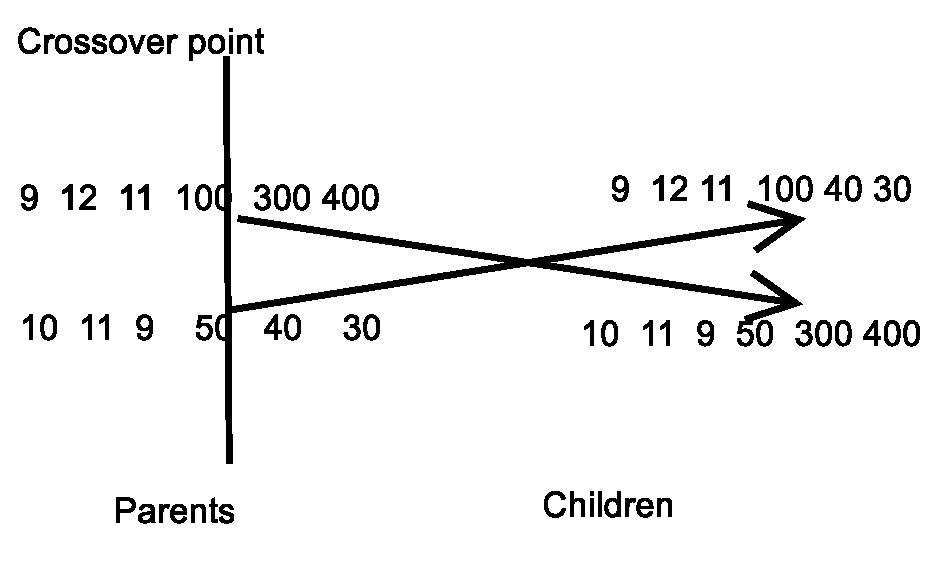
\includegraphics[scale=0.75]{cross}
\end{figure}


\begin{figure}
\caption{Data format.\label{fig:Data-format.}}


D

M

$\begin{array}{ccccc}
x_{11} & x_{12} & \ldots & x_{1D} & y_{1}\\
x_{21} & x_{22} & \ldots & x_{2D} & y_{2}\\
\vdots & \vdots & \vdots & \vdots & \vdots\\
x_{M1} & x_{M2} & \ldots & x_{MD} & y_{M}
\end{array}$
\end{figure}
 
\begin{figure}
\caption{Typical output of the GenClass command\label{alg:Typical-output-of}}

\begin{lyxcode}
~~~1,~~~~~15.43,~~~~~19.32~~~~~

~~~2,~~~~~15.43,~~~~~19.32~~~~~

~~~3,~~~~~15.43,~~~~~19.32~~~~~

~~~4,~~~~~13.71,~~~~~17.05~~~~~

~~~5,~~~~~12.57,~~~~~15.34~~~~~

~~~6,~~~~~12.57,~~~~~15.34~~~~~

~~~7,~~~~~12.57,~~~~~15.34~~~~~

~~~8,~~~~~~~~12,~~~~~13.64~~~~~

~~~9,~~~~~~~~12,~~~~~13.64~

~~FINAL~OUTPUT~EXPRESSION=~if(!(x7<log(cos(cos(((-788.787)+

~~~((sin(x28)/sin(cos(((-7.17)/x34))))+(-83.6))))))|x6>x13\&x7<log(x5)))~CLASS=0.00~

else~~CLASS=1.00~

TRAIN~ERROR~=~12.00\%~

CLASS~ERROR~=~13.64\%~

{*}{*}~CONFUSION~MATRIX~{*}{*}~Number~of~classes:~2~~

~102~~~~3~~~~

~~21~~~50~~

\end{lyxcode}
\end{figure}
\begin{table}
\caption{Parameters for the experiments.\label{tab:Parameters-for-the}}


\begin{centering}
\begin{tabular}{|c|c|}
\hline 
PARAMETER & VALUE\tabularnewline
\hline 
\hline 
$N_{C}$ & 200\tabularnewline
\hline 
$N_{G}$ & 500\tabularnewline
\hline 
$P_{S}$ & $90\%$\tabularnewline
\hline 
$P_{M}$ & $5\%$\tabularnewline
\hline 
\end{tabular}
\par\end{centering}

\end{table}
\begin{table}
\caption{Experimental results\label{tab:Experimental-results}}


\begin{centering}
\begin{tabular}{|c|c|c|c|}
\hline 
DATASET & NEURAL  & RBF & GenClass\tabularnewline
\hline 
\hline 
Wine & 49.55\% & 31.41\% & 8.72\%\tabularnewline
\hline 
Glass & 53.68\% & 50.16\% & 37.72\%\tabularnewline
\hline 
Pima & 27.52\% & 25.78\% & 27.53\%\tabularnewline
\hline 
Ionosphere & 17.08\% & 16.06\% & 9.09\%\tabularnewline
\hline 
EEG & 36.49\% & 66.56\% & 28.60\%\tabularnewline
\hline 
Spiral & 43.23\% & 44.87\% & 41.03\%\tabularnewline
\hline 
Wdbc & 21.03\% & 7.27\% & 6.64\%\tabularnewline
\hline 
Fert & 19.10\% & 12.00\% & 14.10\%\tabularnewline
\hline 
Regions & 34.72\% & 25.78\% & 21.02\%\tabularnewline
\hline 
\end{tabular}
\par\end{centering}

\end{table}

\end{document}
